\section{Theoretische Grundlagen}
\subsection{Biometrie und Biometrische Merkmale}
\subsectionauthor{Torben Brenner}
Bei der Biometrie handelt es sich um die Wissenschaft, die sich mit der Vermessung von biologischen Merkmalen beschäftigt \footcite[Vgl.][]{Sea18}. Dabei werden insbesondere in der Informationstechnologie Technologien zur Messung und Analyse von körperlichen Merkmalen untersucht.\newline
Diese Merkmale werden auch als biometrische Merkmale bezeichnet. Dabei wird unterschieden zwischen den verhaltensbasierten und den physiologischen Merkmalen\footcite[Vgl. ][]{Sas06}. Erstere zeichnen sich dadurch aus, dass eine Person aktiv eine Handlung ausführen muss um das Merkmal zu zeigen, während dem die physiologischen Merkmale dauerhaft von einer Person getragen werden. Ein Beispiel für verhaltensbasierte Merkmale ist die Gangart eines Menschen, die sogar zur Authentifizierung verwendet werden kann\footcite[Vgl. ][]{Cla09}. Ein bekanntes physiologisches Merkmal ist der Fingerabdruck einer Person.\newline
Ein häufiger Einsatzzweck der Biometrie ist die Authentifizierung eines Nutzers gegenüber einem System. Da sich nicht alle Merkmale für eine solche Identifikation eignen, müssen verschiedene Faktoren bei der Auswahl der Merkmale betrachtet werden. \cite{Akj04} nennt zum Beispiel folgende Faktoren: 
\begin{itemize}
	\item \textbf{Universalität}: Jeder Mensch sollte dieses Merkmal besitzen.
	\item \textbf{Unterscheidbarkeit}: Das Merkmal soll sich so stark wie möglich zwischen zwei Personen unterscheiden.
	\item \textbf{Permanenz}: Das Merkmal sollte sich über die Zeit betrachtet nicht oder nur in geringem Maße ändern.
	\item \textbf{Erfassbarkeit}: Das Merkmal sollte möglichst einfach dauerhaft erfasst werden können.
	\item \textbf{Performanz}: Beschäftigt sich mit der Frage mit welchem Zeitaufwand und mit welcher Geschwindigkeit ein Merkmal gemessen werden kann. 
	\item \textbf{Akzeptanz}: Beschäftigt sich mit der Frage in wie weit Nutzer mit der Messung eines Merkmals einverstanden sind. 
	\item \textbf{Umgehbarkeit}: Beschäftigt sich mit der Frage, in wie weit ein Nutzer dem System vortäuschen kann das er ein anderer Nutzer ist.
\end{itemize}
Die ersten vier Faktoren beschäftigen sich im Allgemeinen mit der Eignung eines Merkmals für die Authentifizierung, während sich die letzten Faktoren mit der Eignung eines Biometrischen Systems für eine Aufgabe beschäftigen. Da sich unsere Fragestellung aber nicht auf die Authentifizierung eines Nutzers gegenüber eines Informationstechnischen Systems bezieht, sondern sich mit der Auswertung der erfassten Daten für die Erkennung von Emotionen beschäftigt, ist der Faktor der \textit{Unterscheidbarkeit} zu vernachlässigen. Die restlichen Faktoren werden aber später für die einzelnen biometrischen Merkmale untersucht wobei sich die Faktoren \textit{Performanz, Akzeptanz und Umgehbarkeit} auf die Messung mit Smartphones beziehen.
\subsection{Emotionen}
\subsubsection{Definition}
\subsubsectionauthor{Torben Brenner}
Da wir uns in dieser Arbeit mit der Erkennung von Emotionen beschäftigen, ist es notwendig, dass wir den Begriff der Emotion definieren. Das Problem an dem Begriff der Emotion ist, dass diese ein Hypothetisches Konstrukt ist, welches sich aus der physiologischen Erregung, dem motorischen Ausdruck, Handlungstendenzen und einem subjektiven Gefühl zusammensetzt (\footcite[Vgl.][S.166 Abschnitt Emotion]{Kla02}).\newline
Als Beispiel nennt Klaus Scherer hier das plötzliche Auftreten eines Mannes mit einem Blut verschmierten Messer beim Sonntagsspaziergang. Er beschreibt daraufhin welche Aspekte in diesem Szenario eine Rolle spielen. So kann zum einen eine physiologische Reaktion gemessen werden, in Form eines erhöhten Herzschlages. Außerdem wird eine motorische Reaktion stattfinden, z.Bsp. weit aufgerissener Mund und Augen. Die Handlungstendenz wäre in seinem Beispiel der plötzliche Drang wegzulaufen und bei der späteren Befragung zu dieser Situation könnte eine Person sagen, dass sie Furcht gefühlt hat.\newline
\cite{Kla05} definiert eine Emotion im Zusammenhang mit dem \textit{component process model} als ``eine Abfolge von zusammenhängenden, synchronisierten Veränderungen der Zustände von allen oder den meisten der fünf Subsysteme des Organismus als Reaktion auf die Verarbeitung eines externen oder internen Stimulus Ereignis das relevant für den Organismus ist''\footcite[Übersetzt aus ][S.697 Z.32ff]{Kla05}. In einer Tabelle zeigt Scherer die Verbindung zwischen den Organischen Subsystemen und den Komponenten und Funktionen einer Emotion. 
\begin{figure}[h]
	\centering
	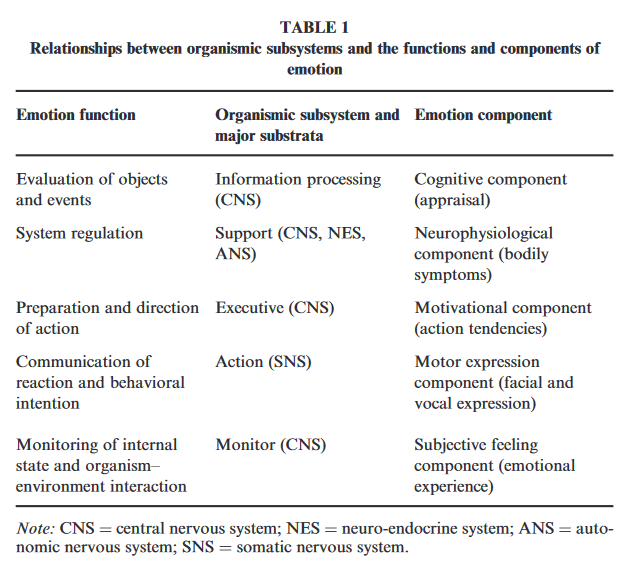
\includegraphics[width=16cm]{Bilder/Relationships-between-organismic-subsystems.png}
	\label{img:Emotion}
	\caption[Relationships between organismic subsystems and the functions and components of
	emotion - Klaus R. Scherer]{Relationships between organismic subsystems and the functions and components of
		emotion - Klaus R. Scherer\footnotemark}
\end{figure}%
\footcitetext[Vgl.][S.698 Table 1]{Kla05}
Anhand dieser Tabelle lässt sich eine Unterscheidung zwischen dem Begriff Gefühl und Emotion durchführen. Der Unterschied ist das ein Gefühl eine einzelne Komponente der Emotion ist, welche erst in Verbindung mit anderen Emotionskomponenten zu einer Emotion führt. 
\subsubsection{Wie lassen sich Emotionen messen?}
\subsubsectionauthor{Torben Brenner}
Nach dem nun geklärt ist wie eine Emotion aufgebaut ist, müssen wir uns die Frage stellen, wie es möglich ist eine Emotion zu messen. Der naheliegendste Ansatz ist zu versuchen, die einzelnen Emotionskomponenten messbar zu machen. Das dies nicht so einfach umzusetzen ist, zeigt die Betrachtung der kognitiven Emotionskomponente. Diese steht im direkten Zusammenhang mit dem zentralen Nervensystem (siehe \ref{img:Emotion} S.\pageref{img:Emotion}). Eine Messung der Veränderungen in diesem System ist äußerst kompliziert und insbesondere in unserem Anwendungsfall nicht möglich. Daher muss ein anderer Ansatz untersucht werden Emotionen zu messen.
\subsubsection{Geneva Emotion Wheel}
\subsubsectionauthor{Torben Brenner}
Das \textit{Geneva Emotion Wheel} baut auf dem Ansatz auf, die Emotionen anhand verschiedener Dimensionen zu bestimmen. In einem Prototyp für das \textit{Geneva Emotion Wheel} (zu sehen in \ref{img:Geneva} S.\pageref{img:Geneva}) werden die beiden Dimensionen \textit{arousal} und \textit{valence} betrachtet.
\begin{figure}[h]
	\centering
	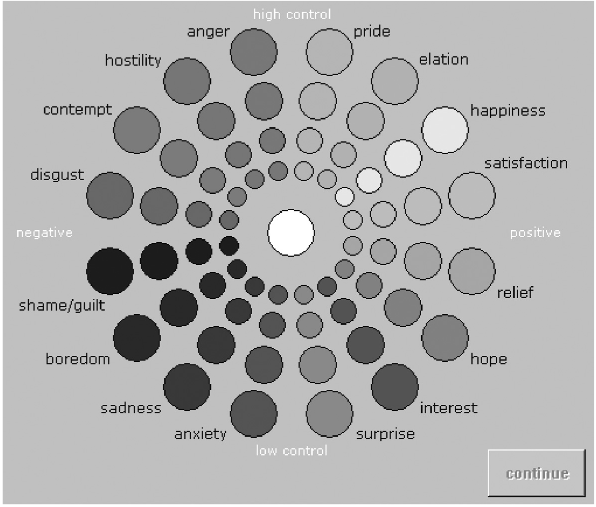
\includegraphics[width=16cm]{Bilder/Geneva-Emotion-Wheel.png}
	\label{img:Geneva}
	\caption[Prototype version of the Geneva Emotion Wheel - Klaus R. Scherer]{Prototype version of the Geneva Emotion Wheel - Klaus R. Scherer\footnotemark}
\end{figure}%
\footcitetext[Vgl.][S.723 Figure 2]{Kla05}
Die erste Dimension bezeichnet wie stark die Erregung eines Individuums ausgeprägt ist in einer Situation. Die zweite Dimension gibt an wie Unwohl sich ein Individuum in einer Situation fühlt. Beide Dimensionen haben gemeinsam, dass sie durch die Befragung eines Individuums ermittelt werden müssen.
\subsubsection{Rad der Emotionen nach Robert Plutnick}
\subsubsectionauthor{Torben Brenner}
Nach dem nun geklärt ist was unter einer Emotion verstanden wird, stellt sich die Frage wie man diese erkennen kann. Das Problem hierbei ist, dass es eine große Anzahl an Emotionen gibt, laut Hokuma\footcite[Vgl.][Absch. 1]{Hok17} sind es 34.000 unterschiedliche Emotionen. Diese verschiedenen Emotionen lassen sich nur schwer erfassen und unterscheiden, weshalb ein Weg gefunden werden muss die Emotionen einzuteilen. Diese Einteilung wurde bereits von Robert Plutchick vorgenommen und herausgekommen sind dabei acht primäre Emotionen: Freude, Traurigkeit, Akzeptanz, Ekel, Angst, Wut, Überraschung und Erwartung.\newline
Mit diesen acht Emotionen hat Plutchick das Rad der Emotionen gebildet(siehe Abbildung).
\begin{figure}[h]
	\centering
	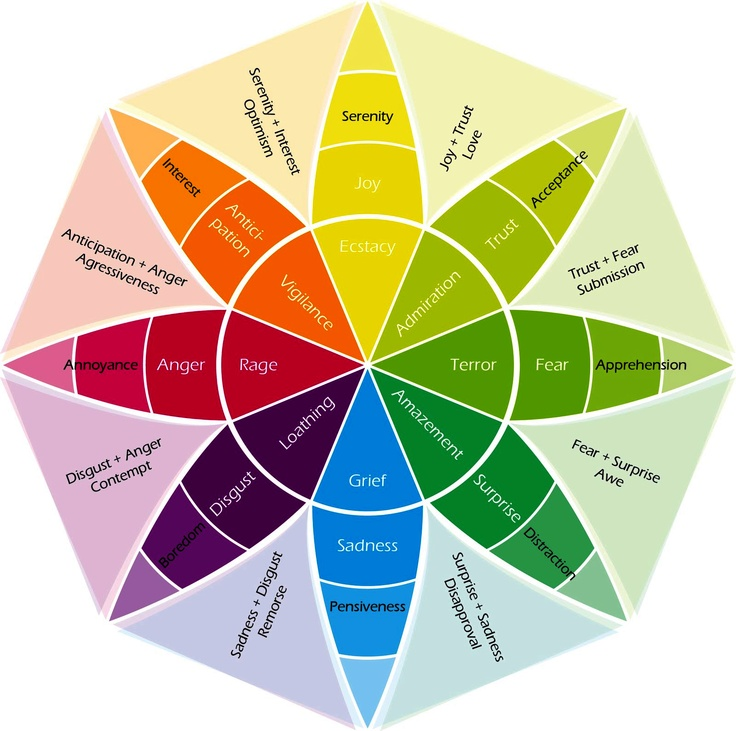
\includegraphics[width=16cm]{Bilder/wheel-of-emotions.png}
	\caption[Rad der Emotionen - Robert Plutchick]{Rad der Emotionen - Robert Plutchick\footnotemark}
\end{figure}%
\footcitetext[Vgl.][]{Hok17}
\newline
Das Rad stellt die primären Emotionen dabei in Relation, wobei die Kombinationen zwischen zwei Emotionen im Raum zwischen diesen steht und Emotionen die gegensätzlich wirken, z. Bsp. Traurigkeit und Freude, jeweils auch gegenüberliegend auf dem Rad sind. Außerdem wird die Stärke einer Emotion durch deren nähe zum Zentrum des Rads gekennzeichnet, z. Bsp. Wut zu toben \footcite[Vgl.][Absch. Elements of the Wheel]{Hok17}.\newline
\subsection{Umgang mit biometrischen Daten}
\subsectionauthor{Torben Brenner}
Eine Problematik, mit der wir uns in dieser Arbeit beschäftigen müssen, ist der Umstand das biometrische Daten nicht immer einen direkten Schluss auf einen Emotion zulassen. So lässt ein hochfrequenter Puls keinen direkten Schluss auf die Emotion zu, die ein Individuum gerade empfindet. Er kann maximal ein Indiz für verschiedene Emotionen sein, z. Bsp. Wut oder Angst. Um mit diesem Umstand umzugehen benötigen wir zwei neue Begriffe die im folgenden genauer erläutert werden. 
\subsubsection{Indiz}
Ein Indiz ist im allgemeinen Sprachgebrauch ein Anzeichen für einen Umstand, an dem sich ein Zustand oder eine Entwicklung absehen lässt\footcite[Vgl.][]{Dud18}. In unserer Arbeit, sehen wir Daten die wir von den Sensoren bekommen, als Indizien an. Ein Indiz macht es wahrscheinlicher bzw. unwahrscheinlicher das ein Individuum eine bestimmte Emotion verspürt. 
\subsubsection{Kausalität}
Als Kausalität wird im allgemeinen der Zusammenhang zwischen Ursache und Wirkung verstanden. In der Physik ist die Kausalität ein grundlegendes Prinzip, welches besagt, ``daß in der Natur nichts ohne Grund passiert, d.h. zu jedem Ereignis (Wirkung) ein anderes (Ursache) existiert, das a) in seiner Vergangenheit liegt und b) zwingende Voraussetzung für das Eintreten der Wirkung ist''\footcite{Sav18}.\newline
In dieser Arbeit werden wir ebenfalls versuchen, kausale Zusammenhänge zwischen Reaktionen des Körpers und den gerade empfundenen Emotionen zu ermitteln.
Ein Werkzeug um kausale Zusammenhänge darzustellen ist in der Literatur der Kausale Graph (im englischen \textit{directed acyclic graph}).
\begin{figure}[h]
	\centering
	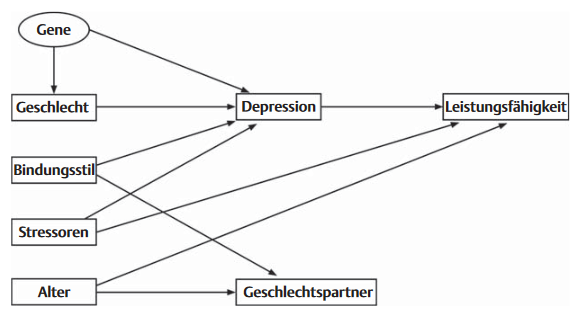
\includegraphics[width=11cm]{Bilder/dag.png}
	\caption[Fiktives Beispiel eines DAGs]{Fiktives Beispiel eines DAGs\footnotemark}
\end{figure}
\footcite[Vgl.][Kausale Graphen - DAGs]{Tho11}
Die Grafik zeigt ein fiktives Beispiel für einen kausalen Graphen. In diesem Beispiel von Thoemmes wird dargestellt das Bindungsstil, Geschlecht, Stressoren und Gene Einfluss auf Depressionen haben. Wichtig ist, dass alle Annahmen die in einem solchen Graph gemacht werden theoretisch begründet werden müssen. Ist dies nicht der Fall, dürfen sie kritisiert und infrage gestellt werden \footcite[Vgl. ][S.3 Kausale Graphen - DAGs]{Tho11}.
\subsection{Emotionsindizien}
\subsubsection{Puls}
\subsubsectionauthor{Torben Brenner}
% Was verstehen wir unter dem Begriff Puls
In diesem Abschnitt beschäftigen wir uns mit dem Puls als ein Indiz für verschiedene Emotionen. Hierbei wird der als der biologische Puls gesehen, das heißt ``die in Abhängigkeit vom Herzrhythmus (Herzmechanik) erfolgende Schwankung von Blutstrom, Blutdruck oder Blutvolumen im Blutkreislaufsystem (Blutgefäßsystem, Blutkreislauf)''\footcite{Spe18}. Neben dieser Definition wird im Lexikon der Biologie auch folgende Definition genannt: ``die vom Herzschlag bewirkte, rhythmisch auftretende Druckwelle (Pulsschlag) in den Arterien''\footcite{Spe18}, welche den Puls als arteriellen Puls definiert. \newline
% Wie wird der Puls gemesen? Ruhepuls nicht Ruhepuls(Sphygmologie)
Es gibt mehrere Möglichkeiten den Puls zu messen. Die häufigste Methode, welche auch in Erste-Hilfe-Kursen gelehrt wird, ist die Messung des Pulses an der Arterie. Das Grundprinzip ist dabei, dass die vom Herzschlag verursachte Druckwelle an der Arterie für Menschen spürbar ist und somit dort mitgezählt werden kann.\newline
% Wie lässt sich der Puls als Biometrisches Merkmal einordnen?
Der Puls ist in der Biometrie als ein physiologisches Merkmal zu sehen. Eine Person muss keine speziellen Handlungen durchführen um einen Puls zu haben. Der Aspekt der \textit{Universalität} ist bei diesem Merkmal gegeben, da jeder Mensch einen Puls besitzt. Eine Erfassung des Pulses ist quasi jeder Zeit möglich, zumindest für Menschen. Ein Smartphone bietet aber auch mehrere Möglichkeiten den Puls zu messen, die später in dem Abschnitt ``Erfassung der biometrischen Daten'' weiter erläutert werden. Der Aspekt der Permanenz ist nicht vollständig gegeben. Der Puls bewegt sich zwar standardmäßig in einem bestimmten Wertebereich, ist aber abhängig von Alter und körperlicher Verfassung einer Person.\newline
% In wie fern kann der Puls als Indiz verwendet werden?
Als Emotionsindiz kann der Puls unterstützend wirken, da dieser eine physiologische Auswirkung von verschiedenen Emotionen sein kann. Dennoch ist er kein alleiniges Merkmal für eine bestimmte Emotion, da sowohl Freude als auch Angst einen erhöhten Puls zur folge haben können.
\subsubsection{Hautleitfähigkeit/Hautwiderstand}
\subsubsectionauthor{Lukas Seemann}
Die menschliche Haut verfügt über \glqq \textit{aktive als auch passive elektrische Eigenschaften, die sich auf Strukturen und Fuktionen der Haut und der in ihr enthaltenen Organe zurückführen lässt.}\grqq{}\footcite[][S. 2]{Bou88} Diese elektrischen Phänomene der Haut sind in wissenschaftlichen Kreisen unter dem Sammelbegriff elektrodermale Aktivität (kurz EDA) bekannt. \footcite[Vgl.][S. 2]{Bou88}
Eine elektrodermale Aktivität, die sich sehr gut als Indikator für Emotionen eignet, ist die Hautleitfähigkeit. Hierzu wird mit einer externen Stromquelle mit geringer Spannung gemessen, wie gut die Haut eines Probanden diesen Strom leitet. \footcite[Vgl. ][S.77]{Moe07} Häufig wird anstand der Hautleitfähigkeit auch der Hautwiderstand gemessen. Diese beiden Indizien stehen in einer negativ proportionalen Beziehung. Dies bedeutet, je höher der Widerstand der Haut ist, desto niedriger ist die Leitfähigkeit und umgekehrt. Letzten Endes sagen beide Indizien dasselbe aus, unterscheiden sich aber in der Betrachtungsrichtung. \footcite[Vgl. ][S. 28]{Die06} \newline
Die Hautleitfähigkeit wird anhand der Menge von Schweiß an den Ausgängen der Schweißdrüßen bestimmt, die sich über den gesamten Körper veteilen. Je mehr Schweiß, der elektrisch sehr gut leitend ist, sich auf der Haut befindet, umso größer ist die Hautleitfähigkeit. Am besten eignen sich  Stellen, an denen die Schweißdrüsen sehr dicht angeordnet sind und die somit sehr schweißsensibel sind. Dies ist zum Beispiel an den Handinnenflächen beziehungsweise Fingerinnenseiten der Fall, die sich deshalb sehr gut für solche Messungen eignen. \footcite[Vgl. ][S.77]{Moe07} 
\begin{figure}[h]
	\centering
	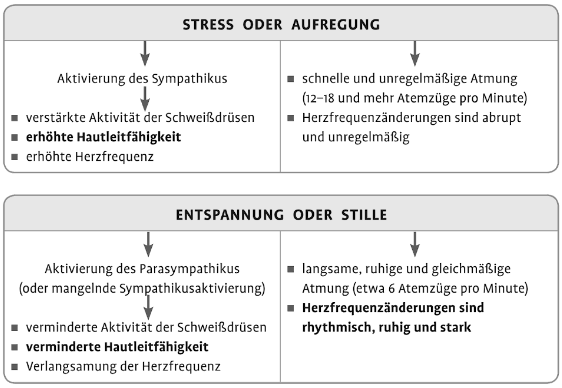
\includegraphics[width=14.6cm]{Bilder/symp.png}
	\caption[Reaktion des Körpers auf Stress und Entspannung]{Reaktion des Körpers auf Stress und Entspannung\footnotemark}
\end{figure}%
\footcitetext[][S. 200]{Dil13}
\newline
\glqq \textit{Die Aktivation beschreibt das Ausmaß der physiologischen Aktiviertheit oder Wachheit eines Menschen}\grqq{}\footcite[][S. 28]{Die06}. Unter Aktivitation versteht man bei Menschen generell jede Art von emotionaler Erregung. Hierzu zählen unter anderem Wut, Aufregung, Schreckmomente oder auch extreme Freude. In Abbildung 3 ist die Reaktion des Körpers auf Stress (darausfolgend auch Aktivation) und auf Entspannung dargestellt. Die Schweißprodukation wird über das unwillkürliche Nervensystem gesteuert. Dieses besteht aus Sympathikus der für die Bereitstellung von Energie und Arbeitsleistungs zustöndig ist, und dem Parasympathikus, der zur Erholung und Wiederherstellung von Körperfunktionen dient. \footcite[Vgl. ][S. 5]{Lie13} \newline Bei Stress oder Aufregung wird der Sympathikus aktiviert, was eine versträkt Schweißproduktion und somit auch eine erhöhte Hautleitfähigkeit hervorruft. Außerdem wird die Herz- und Atemfrequenz erhöht und der Rhymtmus dieser ist unregelmäßig. Die Reaktion auf ein Ereignis, das emotionale Erregung hervorruft, lässt sich meistens innerhalb von einer bis vier Sekunden anhand der Änderung der Hautleitfähigkeit feststellen. \footcite[Vgl.][S. 130f]{Sch14} \newline 
Bei Entspannung hingegen wird der Parasympathikus aktiviert, was zu einer verminderten Aktivität der Schweißdrüßen führt. Die Hautleitfähigkeit sinkt somit auch. Des Weiteren werden Herz- und Atem verlangsamt und gelangen wieder in einen normalen Rhymthmus. \newline
Der Vorteil der Messung der Hautleitfähigkeit ist, dass diese unwillkürlich gesteutert wird und somit keine willentliche Mitarbeit des Probanden erfodert. Da die Aktivierung des Sympathikus automatisch geschieht, kann der Proband die Messung nicht verfälschen. \newline
Ein Nachteil des Verfahren ist, dass die Hautleitfähigkeit nur Rückschlüsse auf den Grad der Aktiviation schließen lässt, jedoch nicht gesagt werden kann, ob es sich um positive oder negative Reaktionen handelt. Die Wut über ein Ereignis würde zum selben Ergebnis führen, wie die übermäßige Freude über ein Ereignis. Aus diesem Grund müssen zur genauen Emotionsbestimmung weitere Indizien herangezogen werden. \footcite[Vgl. ][S.77]{Moe07}
\subsubsection{Mimik}
\subsubsectionauthor{Torben Brenner}
% Was bezeichnet der Gesichtsausdruck
Der Begriff Mimik bezeichnet Bewegungen der Gesichtsmuskulatur mit dem Ziel, eine Emotion auszudrücken. Das nicht jede Gesichtsregung automatisch auch als Mimik gewertet werden kann sieht man beispielsweise beim Kauen \footcite[Vgl. ][Mimik: Eine kurze Definition]{Kar18}.\newline
% In wiefern kann sie als biometrisches Merkmal gewertet werden
Der Vorteil der Mimik als Emotionsindiz ist, dass sie als eines der wenigen Indizien für direkte Aussagen zu den Emotionen gewählt werden kann. So ist es dem Menschen zum Beispiel möglich, alleine durch Beobachtung einer anderen Person Vermutungen anzustellen, welche Emotionen diese gerade empfindet\footcite[Vgl. ][Die sieben Grundemotionen, Absatz 1]{Kar18}. Eine Untersuchung die diese Aussage zusätzlich unterstützt ist der FEEL-Test\footcite[][]{Kes02}. FEEL steht für Facial Expressed Emotion Labeling und ist ein Computerprogramm das auf den Arbeiten von Ekman\footcite{Ekm92} aufbaut. Bei dem Test werden den Probanden Bilder gezeigt die jeweils eine von sechs Basisemotionen wiederspiegeln. Der Proband soll daraufhin versuchen die Emotionen zu erkenne wobei im Ergebnis die Richtigkeit der Antwort und die Antwortzeit betrachtet werden. Ziel des Tests war es ``objektiv
und reliabel die Fähigkeit eines Probanden erfassen, sechs mimisch kodierte Basisemotionen zu erkennen (Freude, Trauer, Ekel, Angst, Überraschung und Ärger)''\footcite[siehe. ][S.5 Z.11ff]{Kes02}. In einer Pilotstudie mit 77 Teilnehmern konnten die Probanden unterschiedlich gut die verschiedenen Emotionen erkennen: ``(Trauer 
70\%, Angst 71\%, Ekel 80\%, Überraschung 84\%, Freude 87\% und Ärger 94\%)''\footcite[siehe. ][S.9 Z.9f]{Kes02}.\newline
Die Ergebnisse der Studie zeigen, dass Menschen aus der Mimik einen Schluss auf eine Emotion ziehen können. Im Verlauf der Arbeit werden wir untersuchen, ob es Möglichkeiten gibt, mit der Smartphonekamera ebenfalls ein solches Ergebnis erzielen können oder dieses sogar übertreffen können. 
\subsubsection{Tippverhalten}
\subsubsectionauthor{Torben Brenner}
Besitzer eines Smartphones verwenden dieses für die verschiedensten Lebensaufgaben. Neben der Hauptaufgabe, dem telefonieren, wird das Smartphone sowohl zum Nachrichten schreiben als auch für das Bilder machen verwendet. Dabei lassen sich theoretisch Daten wie die Tippgeschwindigkeit erfassen, oder aber auch mit Einwilligung des Nutzers der Text versendeter Nachrichten analysieren.
\subsubsection{Gangart}
% Was ist die Gangart
% Auszeichnung als biometrisches Merkmal
% Emotionsindiz?
\subsubsection{Stimme}
\subsubsectionauthor{Torben Brenner}
% Wie entsteht die Stimme
% Stimme als biometrisches Merkmal
% Stimme als Emotionsindiz: Erkennung von Erregung (Acoustic Markers)
Es lässt sich insbesondere die Erregung in der Stimme erkennen --> lässt sich gut zur Unterstützung verwenden 
\subsection{Hardware zur Erfassung von biometrischen Daten}
\subsubsection{Smartphones}
\subsubsectionauthor{Torben Brenner}
% Definition Smartphone
Auch wenn der Begriff des Smartphones heutzutage häufig Synonym zu dem des Mobiltelefons verwendet wird, beschreiben die beiden Begriffe dennoch unterschiedliche Gerätearten. Smartphones sind im allgemeinen eine Weiterentwicklung des herkömmlichen Mobiltelefons. Neben der Standardfunktion des mobilen Telefonierens und der Unterstützung des \textit{Short Message Service} (kurz SMS), bieten Smartphones mittlerweile viele weitere Funktionen wie z. Bsp. GPS oder Internetzugriff\footcite[Vgl. ][S.3 Z.5ff]{Bou11}.\newline
% Unterschied zum herkömmlichen Breitband Telefon/Mobiltelefonen
Dieser erhöhte Umfang an Funktionen ermöglicht es Entwicklern Anwendungen für viele verschiedenen Anwendungsfälle bereitzustellen und somit den Nutzer deutlich besser in seinem Alltag zu unterstützen als mit einem Mobiltelefon\footcite[Vgl. ][Smartphones are tiny Computers]{Ada18}. Eine weitere Entwicklung die vom Mobiltelefon zum Smartphone stattfand, war die Weiterentwicklung des Betriebssystems. Während Mobiltelefone meist mit simplen Betriebssystemen ausgestattet sind, werden Smartphones von komplexen Systemen wie Android oder IOS angetrieben. Diese bieten Nutzern die Möglichkeit zusätzliche Programme zu installieren wie z.Bsp. bei Windows\footcite[Vgl. ][Mobile Operating Systems]{Ada18}.\newline
% Vergleich Leistung mit einem Computer
Der erhöhte Funktionsumfang von Smartphones im Vergleich zu Mobiltelefonen führt uns zur Frage, ob Smartphones auch dazu genutzt werden können, einen Computer zu ersetzen. Verschiedene Hersteller wie z. Bsp. Samsung mit den Dex-Stationen bieten Nutzern bereits die Möglichkeit, ihr Smartphone als PC-Ersatz zu nutzen\footcite{Kai18}. Obwohl Smartphones immer höhere Leistungsspitzen erreichen, werden sie wahrscheinlich auch in Zukunft nicht als vollständiger PC-Ersatz genutzt werden können. Das liegt insbesondere daran das Smartphone CPUs(Central Processing Unit) aufgrund des Formfaktors nicht so gekühlt werden können wie PC-CPUs\footcite[Vgl. ][Power and Heat]{Gav18}.\newline 
% Warum Smartphones zur Emotionserkennung? Ermöglichen Tagesanalyse/Verbreitung
Nun kommen wir zu der Frage warum wir Smartphones verwenden wollen um Emotionen zu erkennen. Zum einen sind Smartphones in der Lage, durch verschiedenen verbaute Sensoren zu sehen, fühlen und zu hören\footcite[Vgl.][S. 1 Abs. 2]{Bie14}. Wie in dem Artikel beschrieben, geben uns die verbauten Sensoren enorme Möglichkeiten mit dem Smartphone die Umwelt wahrzunehmen. Wie leistungsfähig die verschiedenen Komponenten mittlerweile geworden sind, zeigt Apple mit dem IPhone X, welches mithilfe der Kamera und Infarotsensoren, die Veränderungen von Gesichtszügen erkennt und auf sogenannte Animojis überträgt\footcite[Vgl. ][Animoji: So funktioniert es]{Com17}. Ein weiterer Grund aus dem wir die Emotionserkennung mit Smartphones untersuchen wollen ist die Tatsache, dass Smartphonenutzer ihr Gerät häufig rund um die Uhr bei sich tragen. Dies ermöglicht es für verschiedene Anwendungsszenarien eine Überwachung der Emotionen des Nutzers über den Tag hinweg durchzuführen.
\subsubsection{Sensoren}
\subsubsectionauthor{Torben Brenner \& Lukas Seemann}
Sensoren dienen zur Erfassung eines physikalischen Zustandes und der Transformation dieses Zustandes in einen Impuls der verarbeitet werden kann\footcite[Vgl.][]{Web18}. In der Computertechnik, dienen Sensoren häufig dazu, den physikalischen Zustand verständlich für einen Computer zu machen, in dem dieser in einen Datensatz umgewandelt wird. \newline 
%Ursprünglich aus anderem Kapitel hizugefügt
Die bereits in Kapitel 2.4.2 beschriebene elektrodermale Aktivität kann mithilfe von EDA-Sensoren gemessen werden. Diese Art von Sensoren sind üblicherweise nicht in Smartphones eingebaut, weswegen die Hautleitfähigkeit mit externer Hardware gemessen werden muss. \newline
Die für heute eher unübliche Messungsart der elektrodermalen Aktivität stellt die endosomatische Messung dar. Indem winzige Elektroden in die Haut eingestochen werden, kann die Aktivität der Nerven in der Haut gemessen werden. \footcite[Vgl.][Folie 25]{Sch12} Hierbei handelt es sich jedoch nicht um eine Messung der Hautleitfähigkeit sondern um eine Messung des Hautpotenzials. \newline
Bei der exosomatischen Messung hingegen wird ein schwacher Strom von ungefähr 0.5 Volt an die Haut angelegt. Die Spannung wird hierbei konstant gehalten, wodurch die Leitfähigkeit der Haut gemessen werden kann. Hierbei gemessen wird entweder in der Einheit Siemens für den elektrischen Leitwert oder in Ohm für den Widerstand. Die Elektroden des Sensor sind meistens aus Silber oder Silberchlorid und werden meist an zwei Stellen der nicht dominanten Hand angebracht. \footcite[Vgl.][Folie 25]{Sch12} Wie in Abbildung ? dargestellt gibt es verschiedenen Möglichkeiten der Handinnenfläche, die gut geeignet sind, (\#1, \#2 oder \#3). \newline 
\begin{figure}[h]
	\centering
	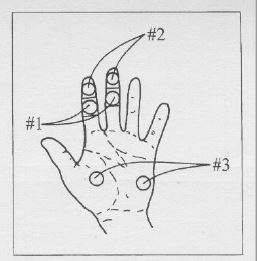
\includegraphics[width=12cm]{Bilder/gsr-hand.jpg}
	\caption[Positionsmöglichkeiten der EDA-Messung]{Positionsmöglichkeiten der EDA-Messung\footnotemark}
\end{figure}\footcitetext[][Folie 25]{Sch12}
\newline
Diese Art von Sensoren sind die heutzutage übliche Vorgehensweise bei EDA-Messungen. Häufig sind sie auch unter dem Namen GSR-Sensor\footnote{GSR: Galvanic Skin Response} bekannt und darunter im Internet erhältlich. GSR-Sensoren sind als Modul für den Mikrocontroller Arduino verfügbar.\footcite[beispielsweise:][]{Gro18} Dies stellt eine Möglichkeit dar, einem mobilen Endgerät die Sensordaten zum Beispiel über Bluetooth oder WiFi zur Verfügung zu stellen. In Abbildung ? ist ein GSR-Sensor inklusive der Elektroden für die Fingerinnenseiten, der mit Arduinos kompatibel ist, abgebildet.
\begin{figure}[h]
	\centering
	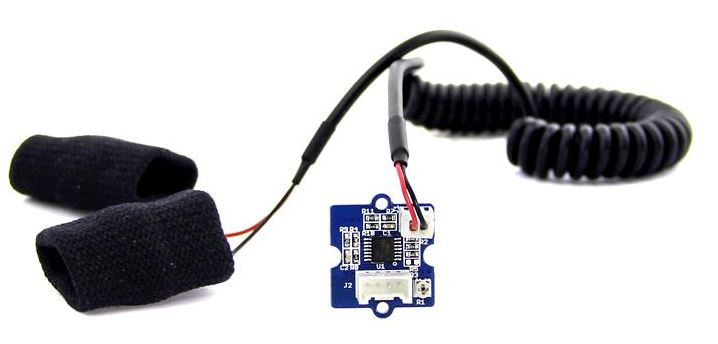
\includegraphics[width=15cm]{Bilder/sensor.jpg}
	\caption[GSR-Sensor mit Finger-Elektroden]{GSR-Sensor mit Finger-Elektroden\footnotemark}
\end{figure}%
\footcitetext{Gro18}
